\section{Results and Discussion}
We computed correctness of our DA subjects in identifying the missing information by using the Sorensen-Dice coefficient~\cite{sorensen1948method}, and show these values in Figure~\ref{fig:barchart}. We found that offline analysts were just slightly more accurate than real-time analysts, and that both groups faired well. Offline users were significantly more accurate solving DA\_Task 4 (i.e., identifying the recommended movie) since the two groups differed in how they approached this task. Offline users located their users' recommendation tasks, then picked one of the last movies users viewed, since they were more likely to be an end-answer; real-time users quickly identified when a recommendation task started and rushed to pick movies that their users considered early on. The real-time analysts also tended to be less accurate in detecting transitions between tasks. Finally, offline users seemed more observant of the actual heatmap values, while real-time users reported that they focused mainly on the sorted labels on the sides. 

While our preliminary results are promising, we acknowledge that our analysts monitored only a few concurrent users. Even so, we provide a first account of how DOI eye-tracking can be used to enable real-time tracking of users' visual interests, and provide a stepping stone for applications described in Section~\ref{sec:Introduction}.  Moreover, we believe more complex visualizations that borrow encoding principles and functionality from time-line and event monitoring applications, could allow analysts to track many users at once. This is supported by one of our approach's main advantages: the ability to track users' eye-tracking data without having to look at the visual stimuli they viewed; this allows us to stack compact visualizations of multiple users' data, and pose complex computational queries.  



\begin{figure}[htb]
  \centering
  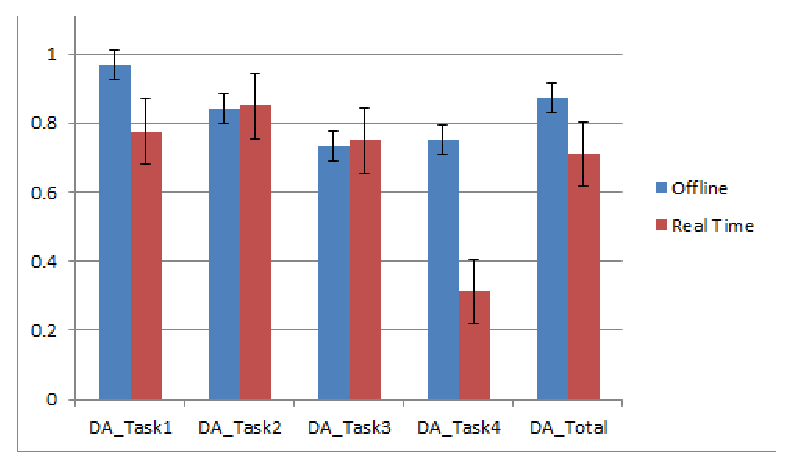
\includegraphics[width=0.9\linewidth]{images/barchart.eps}
  \caption{Barchart diagram showing the correctness of offline users vs real-time users.}
	\label{fig:barchart}
\end{figure} 

